% \section{Motivation}
% \label{sec:motivation}

% - Scholarly Literature Search is time-consuming and cognitively demanding, nowadays all research findings are communicated via digital scholarly articles, a practice often referred to as the document-centric approach \cite{jaradeh_open_2019-1,auer_towards_2018}
% - Research Knowledge Graphs can help to make research more efficient
% - But to query information from the graph is also demanding as the user is required to know the graph structure to traverse the graph to find related information 
% - Recent development in the literature unifies LLMs with Graphs to exploit the advantages from both: 
% -- LLM Advantages: General Knowledge, Language Processing, Generalizability
% -- Graph Advantages: Structural Knowledge, Accuracy, Deciseveness, Interpretability, Domain-specific Knowledge, Evolving Knowledge
% - Graph Retrieval Augmented Generation (GraphRAG) \cite{peng_graph_2024} has been established which utilizes LLMs to retrieve relevant knowledge from the graph given a natural language question
% - As shown by current approaches, adding a Graph to the Retrieval can improve the quality and reliability of answers generated by LLMs \cite{edge_local_2024, guo_lightrag_2024}
% - Most current graph retrieval approaches focus on general domains and it is unknown how they perform in the scholarly literature search task
% - However some research is starting on the scholarly domain \cite{jaradeh_question_2020,taffa_leveraging_2023,giglou_scholarly_2024}


% Need to add somewhere:
% - We developed a question taxonomy that with the goal: “The taxonomy is designed to classify the characteristics of questions posed to KGQA retrieval systems in the literature search domain, enabling the creation of diverse question sets that test a broad range of retrieval capabilities.”
% - We created HubLink, a new retrieval approach that leverages the structure of RKGs to improve the relevance and accuracy of retrieved contexts and be able to answer complex questions that are asked in the literature search.
% - We evaluated against baselines that are training free (as our approach) which means that they use pre-trained LLMs and do not require further fine-tuning or training of models. \cite{jiang_structgpt_2023}, \cite{sun_think--graph_2024}, \cite{wen_mindmap_2024}, \cite{sui_fidelis_2024}, \cite{baek_direct_2023}
% - Approaches like semantic parsing struggle because of: Semantic Parsing hat allerdings zwei bedeutende Herausforderungen wie von \textcite{gu_knowledge_2022} herausgestellt: \emph{Schema-Level Complexity} und \emph{Fact-Level Complexity}. Zunächst ist das Schema eines modernen \gls{kg} extrem reichhaltig was bedeutet, dass die Anzahl an Items eines Schemas mehrere tausend beinhalten kann. Beispielsweise hat der FREEBASE \gls{kg} über 8k an Schema items. 
% - Klar machen warum es sinnvoll ist das man Knowledge Graphen verwendet statt einfach direkt die Informationen zu embedden -> Auf Die Paper LightRag und MicrosoftGRAPH rag \cite{edge_local_2024, guo_lightrag_2024} verweisen die das zeigen. Also im Prinzip ist es in der Motivation schonmal wichtig klar zu machen warum der Ansatz gebraucht wird. Also das Sparql Generierung nicht aussreicht und das nur das Document Embedding auch nicht reicht

Today, almost all scholarly findings are communicated through digital scholarly articles, a practice often referred to as the document-centric approach \cite{jaradeh_open_2019-1,auer_towards_2018}. Although the transition from print to digital has significantly improved accessibility \cite{sompel_all_2009,bosman_scholarly_2017}, it still does not fully take advantage of modern digital technologies. In current research practice, each publication is treated as an isolated unit of knowledge, making it challenging to interlink related findings, methodologies, and underlying data. This isolation becomes especially problematic given the exponential growth of scientific literature \cite{bornmann_growth_2021}. Researchers must navigate an extensive body of text to identify relevant insights. This process is challenging due to the sheer volume of content and also the addition of inherent issues that plague text searches. For example, the lexical gap problem, in which misspellings, synonyms, abbreviations, ambiguous words, and the ignored word order hinder the effectiveness of searches \cite{li_unsupervised_2022}. Consequently, literature search becomes a time-consuming and cognitively taxing process, requiring careful crafting of search queries, manual sifting through countless documents, and painstaking synthesis of scattered evidence. 

Recently, \glspl{llm} have demonstrated powerful capabilities in understanding natural language, expressiveness, general knowledge, and generalization \cite{yang_give_2024}. In the context of \gls{qa}, integrating \glspl{llm} allows users to pose queries in natural language, with the system generating relevant answers. This is particularly interesting for scholarly literature search as it allows researchers to find answers to scientific resources by asking questions in natural language, effectively reducing manual effort. However, using the pre-trained internal knowledge of the \glspl{llm} is not sufficient because their answers may lack depth, be subject to hallucinations, and do not provide transparency regarding the underlying reasoning process \cite{yang_give_2024}. 

To mitigate these issues in the \gls{qa} setting, \gls{rag} has emerged, in which an external \gls{kb} is used to provide relevant context to the \gls{llm} to enhance the answer generation \cite{lewis_retrieval-augmented_2021}. In this framework, an indexing phase takes place where the collection of documents is split into text chunks, which are then converted into dense vector representations and stored in a vector store. At query time, the vector representation of the question is used to conduct a distance-based search in the vector space to find the most relevant text chunks. Although this approach can be applied to the scholarly literature search setting \cite{lu_dense_2024}, naive \gls{rag} encounters notable drawbacks. Retrieval can suffer from poor precision and recall, missing crucial context, or retrieving irrelevant information \cite{gao_retrieval-augmented_2024}. Furthermore, \glspl{llm} often struggle with noisy or misleading documents, fail to abstain from answering when relevant information is absent, perform poorly at integrating information across multiple sources, and are prone to accepting factual errors in the retrieved context \cite{chen_benchmarking_2023}.

An alternative to document-centric knowledge representation is to structure and interconnect representations of scholarly knowledge \cite{jaradeh_open_2019-1}. This can be achieved using \glspl{kg} where knowledge is curated from structured and unstructured sources \cite{verma_scholarly_2023}. Specifically for the academic domain, these graphs are referred to as \glspl{rkg} and offer a promising solution to structure and interlink scholarly information. With the aim of transforming scientific communication from document-centric to knowledge-centric \cite{auer_towards_2018}, \glspl{rkg} provide a structured and machine-readable representation of scholarly knowledge by taking into account the relationships between texts and the incorporation of structural information as additional knowledge \cite{peng_graph_2024}.

The unification of \glspl{llm} and \glspl{kg} is a relatively new research field that aims to utilize the advantages of both in various applications \cite{pan_unifying_2024}. One such application is \gls{kgqa}, where the integration of knowledge from a \gls{kg} to inform the \gls{llm} during inference is investigated \cite{banerjee_knowledge_2024,chakraborty_introduction_2021,chakraborty_introduction_2019,pan_unifying_2024,yani_better_2022,peng_graph_2024,jin_large_2024,feng_trends_2023,li_survey_2024,agrawal_can_2024,procko_graph_2024}. 
Although many \gls{kgqa} approaches have emerged, most of the approaches are focused on open-domain \gls{qa} and have not yet been tested in the scholarly field. Furthermore, approaches explicitly aimed at the scientific field focus primarily on \gls{sp} methods that automatically create structured queries from natural language queries using training examples \cite{banerjee_dblp-quad_2023, taffa_leveraging_2023, lehmann_large_2024, jiang_structure_2023, jaradeh_question_2020}. 

Despite being effective in controlled settings, \gls{sp} methods struggle to adapt to dynamically evolving \gls{kg} schemas, leading to poor performance when encountering previously unseen entities or relations. In addition, semantic parsing approaches face significant scalability challenges, including both schema-level and fact-level complexities \cite{gu_knowledge_2022}. These problems are exacerbated by the extensive schema richness of modern \glspl{kg}, which often encompasses thousands of schema items. Moreover, semantic parsing methods typically require manually curated training datasets, which are costly to produce and limit their applicability in real-world research environments, making the methods inconvenient to use. 

Consequently, we identify a research gap in applying alternative \gls{llm}-based strategies to the scholarly \gls{kgqa} task. Most alternative strategies are developed and evaluated on general-purpose graphs like Freebase or Wikidata \cite{peng_graph_2024}. However, these approaches cannot be easily adapted to the scholarly domain \cite{saikh_scienceqa_2022}. Moreover, current retrieval approaches often ignore the source diversity of retrieved information, potentially returning multiple pieces of information from the same publication, reducing the breadth of evidence needed for robust scholarly inquiries. Therefore, the scholarly domain remains underexplored within \gls{kgqa} research.

Motivated by these challenges, we argue that research on scholarly \gls{kgqa} should explore directions beyond semantic parsing to develop methods that do not require training or fine-tuning and can adapt to dynamically changing \gls{kg} schemas. Our thesis contributes a novel \gls{kgqa} retrieval approach that complies with the above-mentioned criteria. We rigorously evaluated the approach on a scholarly literature search task in a \gls{swa} setting against five state-of-the-art baseline \gls{kgqa} approaches on the \gls{orkg} to demonstrate its superiority in retrieval performance. We further contribute a new taxonomy for the classification of questions querying \gls{kgqa} systems for literature search. With these contributions, our aim is to advance research in the direction of \gls{kgqa} in the scholarly literature search domain.


% In summary, despite promising advances in \gls{grag} and \gls{kgqa}, the academic domain remains underexplored. Existing methods either depend on general purpose graphs that fail to capture the specific request of literature search or rely on semantic parsing methods that struggle with evolving and scaling \gls{kg} schemas. Therefore, more research is required to achieve a robust, scalable, and schema-agnostic retrieval approach tailored for scholarly \glspl{kgqa}.

% Although helpful, this document-centric approach still struggles with precision and recall in \gls{qa} tasks \cite{gao_retrieval-augmented_2024}.

% By encoding semantic and relational information, \glspl{rkg} facilitate sophisticated queries and structured retrieval that surpass traditional keyword-based methods. 

% Despite these advantages, effectively querying an \gls{rkg} remains challenging. Traditional methods such as manually crafting SPARQL queries require users to possess in-depth knowledge of the graph schema. Even with user-friendly interfaces like that of the \gls{orkg} \cite{jaradeh_open_2019}, navigating these graphs can be cumbersome, particularly for complex queries.


% into the \gls{rag} framework, forming what is now known as \gls{grag} \cite{peng_graph_2024, pan_unifying_2024}. \gls{grag} approaches leverage the structured, relational nature of \glspl{kg} to retrieve more relevant and interpretable contexts. A growing body of research demonstrates the effectiveness of these methods in various domains \cite{pan_unifying_2024,peng_graph_2024,jin_large_2024,feng_trends_2023,li_survey_2024,agrawal_can_2024,procko_graph_2024}.



% Furthermore, we observe that many current retrieval approaches require additional training or fine-tuning prior to the retrieval process. 
% This is a significant limitation, as it requires ground truth data, which is often unavailable. 
% We envision, that for useability in practice, a retrieval approach should be \enquote{plug-and-play}, meaning that it should not require any training or fine-tuning prior to the retrieval process. 
% As such, \emph{the approach should only require the \gls{rkg} and no additional ground truth data}. 


% Moreover, we identified that many current retrieval approaches are only considering the retrieval of single entities as oposed to complex natural language answers.

% Researchers are confronted with the task of navigating the immense growth of scientific literature \cite{bornmann_growth_2021}, which is made even more difficult as there is no dedicated database for scientific literature. As consequence, researchers have to use academic search engines to find relevant literature. 

% Traditional results from search engines include a list of links to information sources that may contain the answer to the question of the user. However, this approach requires cognitive effort from the user to collect the needed information from the individual search results. To relieve users of this effort, the design of result presentation from search engines has changed with the introduction of \glspl{llm} as illustrated in \autoref{fig:new_search_engine_results_page}. Instead of providing a list of links, the search engine now provides textual answers each linked to the source of the information \cite{gienapp_evaluating_2024}.

% \begin{figure}
%     \centering
%     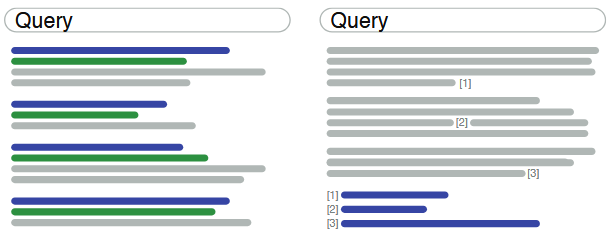
\includegraphics[width=1.0\linewidth]{figures/new_search_engine_results_page.png}
%     \caption{Change of results presentation in search engines \cite{gienapp_evaluating_2024}}
%     \label{fig:new_search_engine_results_page}
% \end{figure}

% The research community has proposed many QA systems, but to the best of our knowledge none focus on scholarly knowledge \cite{jaradeh_question_2020}

% TODO ADD Semantic Parsing Discussion:

% Semantic Parsing methods are early adopters for \gls{qa} on \glspl{kg}. These methods convert questions into a structural query such as SPARQL

% However, these methods heavily rely on the quality of generated queries. If the query is not executable, no answer will be generated. \cite{sui_fidelis_2024}
% Most important: Knowledge Base Question Answering: A Semantic Parsing Perspective
% Auch nochmal schauen warum Embeddingbasierte Ansätze Probleme hat
% Klar machen warum es sinnvoll ist das man Knowledge Graphen verwendet statt einfach direkt die Informationen zu embedden -> Die Paper LightRag und MicrosoftGRAPH rag verweisen die das zeigen. Also im Prinzip ist es in der Motivation schonmal wichtig klar zu machen warum der Ansatz gebraucht wird. Also das Sparql Generierung nicht aussreicht und das nur das Document Embedding auch nicht reicht